\documentclass[%
%reprint,
%superscriptaddress,
%groupedaddress,
%unsortedaddress,
%runinaddress,
%frontmatterverbose, 
preprint,
%showpacs,preprintnumbers,
%nofootinbib,
%nobibnotes,
%bibnotes,
amsmath,amssymb,
aps,
%pra,
prb,
%rmp,
%prstab,
%prstper,
floatfix,
]{revtex4-1}


\usepackage{graphicx}% Include figure files
%\usepackage{dcolumn}% Align table columns on decimal point
\usepackage{bm}% bold math
\usepackage{amsmath}
\usepackage{subfigure}

\begin{document}

\preprint{Version 0.5.1}

\title{SMMP: A Secure Multi-Party Messaging Protocol}% Force line breaks with \\

\author{David R. Andersen}
 \email{k0rx@uiowa.edu}
 \altaffiliation[Also at ]{Department of Physics and Astronomy, The University of Iowa.}%Lines break automatically or can be forced with \\
\author{Mark S. Andersland}
 \affiliation{Department of Electrical and Computer Engineering, The University
 of Iowa, Iowa City, IA 52242}
\author{Tycho J. Andersen}
 \affiliation{Canonical, Inc.\\ Madison, WI 53703}

\date{\today}% It is always \today, today,
             %  but any date may be explicitly specified

\begin{abstract}
We describe a new secure, multi-party, synchronous communication protocol.
The protocol follows a peer-to-peer model and provides perfect forward
secrecy and perfect future secrecy against a computationally-bounded adversary,
as well as information-theoretic plausible deniability for participants in
a multi-party conversation.
The protocol uses a three-round, authenticated Burmester-Desmedt group key agreement
protocol to generate a shared secret between a group of $N$ participants.
Conversation participants authenticate to each other
during key agreement via a triple Diffie-Hellman mechanism.
Individual message keys are updated after receipt of each message by incorporating
new key material distributed by the sending participant.
No security requirements are imposed on the underlying transport layer, and
our protocol leaks no metadata beyond that exposed by the transport layer.
Conversation transcript universality is assured by a conversation digest that is updated
upon receipt of each message, and all conversation messages are signed to
verify proof of origin.
All setup operations prior to group key agreement take place over an insecure
channel.
SMMP represents a significant improvement in security and efficiency over
current secure, multi-party messaging protocols including GOTR, mpOTR, and
improved GOTR.
\end{abstract}

\pacs{73.20.Mf}% PACS, the Physics and Astronomy
                             % Classification Scheme.
%\keywords{Suggested keywords}%Use showkeys class option if keyword
                              %display desired
\maketitle

%\tableofcontents
\section{\label{sec:Introduction}Introduction}
Secure multi-party messaging has been an elusive goal of security researchers
for a long time. The initial group off-the-record (GOTR) `virtual server'
approach\cite{ref:bian} was deemed unsatisfactory
because it has the unfortunate drawback of not permitting all participants to
confirm that they are receiving unmodified copies of all messages.
A further attempt to solve this problem\cite{ref:goldberg} was incomplete
because of the lack of a simple, secure key-agreement
strategy. Work on the problem
continues to date, most notably with\cite{ref:cryptocat}.
Liu \textit{et.al.}\cite{ref:liu}
recently improved the security of GOTR/mpOTR using a Burmester-Desmedt group
key agreement mechanism imposed on top of a network comprised of binary
encrypted channels between participants.

In this paper, we describe a novel secure multi-party messaging protocol (SMMP) with a
simple key-agreement algorithm that provides perfect forward secrecy (PFS) and
perfect future secrecy (PFuS) against a computationally-bounded adversary,
as well as information-theoretic plausible deniability (PD) for participants
in a group conversation. Our protocol
is a peer-to-peer protocol, whereby each participant (peer) contributes new
key material to the group key set with each message sent.
This key-update mechanism is called a ratchet.
In contrast to the various mpOTR/GOTR proposals, no constraints on the security
of the underlying transport layer are required during key agreement or otherwise.

SMMP makes use of six underlying cryptographic primitives, namely: 1) an
underlying (unspecified) symmetric encryption algorithm, 2) the elliptic-curve
Diffie-Hellman key agreement protocol, 3) the finite-field Diffie-Hellman key
agreement protocol, 4) a secure cryptographic hash function, 5) a secure
cryptographic message authentication code, and 6) a secure key-derivation
function.

\section{\label{sec:keypoints}Key Points}
\begin{itemize}
\item Burmester-Desmedt\cite{ref:burmester} group key agreement
takes place using finite-field, cyclic-group
Diffie-Hellman key agreement as the underlying protocol.
\item Participants authenticate each other during group key agreement via a
triple Diffie-Hellman mechansim.
\item During the conversation, elliptic curve Diffie-Hellman key operations
are performed, minimizing the required key-exchange bandwidth.
\item The protocol is synchronous. A method for resynchronizing those
participants that lose synchronization due to lost packets from collisions or
transport failure is included in the protocol.
\item Group setup is via an insecure channel.
\item No security constraints are imposed on the underlying transport layer.
\item Participants may be added to the group via a reinitialization of the
group secret. A participant may leave the group by simply stopping
participation and not updating his ratchet state.
\item A uniform message transcript is assured over all participants via a
conversation digest that is updated with each message. If the digest does not
match what a receiver expects, a resynchronization of the protocol is requested.
\item The underlying symmetric encryption algorithm used for communication is
unspecified.
\end{itemize}

\section{\label{sec:background}Background}
Various protocols exist for facilitating secure one-to-one messaging, including
Off the Record Messaging (OTR)\cite{ref:otr1,ref:raimondo,ref:otr2,ref:otr3,ref:otr}, Silent Circle Instant Messaging Protocol
(SCIMP)\cite{ref:scimp}, and Axolotl\cite{ref:axolotl}. Each of these protocols
provides security through the use of ephemeral keys for symmetric encryption.
The method of generating and exchanging these keys varies widely between the
three protocols. All of the protocols provide forward
secrecy. Some also provide plausible deniability, and one (Axolotl) also
provides perfect future secrecy (compromise of the current keyset does not cause
compromise of future keysets). However, each of these protocols is limited to
the one-to-one messaging case.

OTR was the first such protocol. It is based on an Advertise $\rightarrow$
Acknowledge $\rightarrow$ Use method for key updating. OTR has been widely used
for secure instant messaging and applications containing OTR plugins are
available for XMPP, IRC, and other messaging systems.

SCIMP is a proprietary protocol developed by Silent Circle as their solution for
providing secure communications as part of their product line. The key
advancement algorithm for SCIMP is essentially a hash. Each symmetric encryption
key is hashed to obtain the key for the next ratchet step. As a result, a key
compromise at any point will permit an attacker to follow the conversation from
that point on.

Axolotl is the first one-to-one messaging protocol to provide future secrecy. In
this protocol, randomly-generated key data is mixed in to the ratchet state with
each message send/receive operation, so that a compromised keyset permits an
attacker access to only one message. Following the conversation requires a new
key compromise with each message sent.

The first proposal for a secure group $(N > 2)$ messaging protocol was that of
Bian \textit{et.al.}\cite{ref:bian} [Group Off The Record (GOTR)].
The protocol is based on a virtual server,
a participant that sets up a secure one-on-on channel with each member of the group.
When members of the group who are not the virtual server wish to communicate
with each other, they relay their messages through the virtual server. Several
problems with this approach were identified. First, the virtual server must be
assumed honest. The virtual server handles decryption/reencryption from one user
to another, as well as authentication of all group members. As a result, a
dishonest server (or compromise of the server) would be catastrophic to the
security of the group conversation. Second, the protocol leaks metadata.
High-level addressing data is sent in plaintext. And finally, there is no mechanism for
conversation transcript verification. As a result of these problems with GOTR, a
better solution was necessary.

A second proposal for a secure group messaging protocol was made by Goldberg
\textit{et.al.}\cite{ref:goldberg} [multi-party Off The Record (mpOTR)].
While this protocol solves some of the
problems associate with the Bian messaging scheme, it has additional problems
and is not a good solution. In particular, mpOTR provides PD against offline
judges only. Further, it links all messages in a given transcript together,
meaning that if an honest user commits to authoring or participation in a part
of the transcript, they have committed to the entire transcript. Also, as with
all OTR-based protocols, PD is achieved by publishing ephemeral keys
post-conversation. Finally, the group encryption key is not automatically
updated in mpOTR, and as a result, PFS is not guaranteed - a ``window of
compromise" exists.

An improvement of the security of the mpOTR/GOTR protocol was made by Liu
\textit{et.al}\cite{ref:liu} using Burmester-Desmedt\cite{ref:burmester}
for group key agreement. The improved mpOTR/GOTR requires an
underlying network of secure, binary communication channels that exist between
participants.
Complexity of this improved mpOTR/GOTR protocol is an issue. For each group key
update, a total of six rounds of group key agreement exchanges are required.
Further, each participant must maintain the status for $2(N-1)$ virtual nodes.
Thus, group key agreement is a computationally-intensive task that
may preclude conversation participants from updating their encryption keys on a
per-message basis. Finally, as with all OTR-based schemes, publication of the
ephemeral signing keys at the end of the conversation is required to facilitate
PD.

In this paper, we present a secure, peer-to-peer multi-party messaging protocol
(SMMP) that provides PFS, PFuS, and PD, and has a simple key agreement
algorithm requiring three exchanges to complete key agreement (including
authentication between all peers - see Fig. \ref{fig:exchange}).
The protocol allows all group members to confirm that they are
receiving a complete transcript of the group conversation, and provides a
robust mechanism for resynchronization of the ratchet state if messages are lost
(\textit{e.g.} because of failure of the underlying transport mechanism).

\section{\label{sec:notation}Notation}
The following notation is used:
\begin{itemize}
\item $N$ is the total number of participants in the group (including the
Organizer)
\item $\oplus$ is the bitwise XOR operator
\item $\{N_i\}$ is the set of all $N_i$ and $\{N_i\}_m = N_m$.
\item $\mathcal{\hat{A}}_i$ is the ratchet state for
participant $P_i$.
\item $||$ is the concatenation operator
\item $||_i \, x_i$ means concatenation of all $x_i$ running from the smallest
to the largest index $i$
\item Lower case keys are private ECDH (or DH in the case of the group
key-agreement handshake) keys.
\item Upper case keys are public ECDH (or DH in the case of the group
key-agreement handshake) keys.
\item hash() is a secure, one-way cryptographic hash function.
\item mac$(k,m)$ is a secure message authentication code that
authenticates a message $m$ using key $k$.
\item KDF() is a secure key derivation function, \textit{e.g.} pbkdf2.
\item $c = e(k, m)$ and $m = d(k,c)$ are the underlying (unspecified) symmetric
encryption and decryption algorithms that use a key $k$ to transform a plaintext
$m$ into ciphertext $c$ and \textit{vice versa}.
\item MK is a master key from which the initial ratchet state
$\mathcal{\hat{A}}_i$ is computed by each participant $P_i$. This parameter is
securely erased after computing the initial ratchet state.
\item $X$ is the generator for the elliptic curve and ECDH() is the Diffie-Hellman
operator on the elliptic curve, \textit{i.e.}, for private key $u$, the
corresponding public key is $U = \mathrm{ECDH}(u, X)$. The shared secret between
$y$ and $z$ is then $ \mathrm{ECDH}(y,Z) = \mathrm{ECDH}(z,Y) =
\mathrm{ECDH}(y,\mathrm{ECDH}(z, X))$.
\end{itemize}

\section{\label{sec:protocolstate}Protocol State}
Each Participant $P_j$ will maintain the following state variables in persistent
storage:
\begin{itemize}
\item RK - the root key
\item mk - the message key
\item $v$ - the group private key
\item $\mathrm{conv\_digest}$ - the digest of all conversation messages so far
\item $r_j$ - the participant private ratchet key (for participant $P_j$,
$\mathrm{ECDH}(r_j, X) = R_j$)
\item $r_j^{init}$ - the initial value of participant $P_j$'s private ratchet
key
\item $\{R_i\}$ - the set of public ratchet keys from each participant $P_i$
\item $\{R_i^{init}\}$ - the set of initial values of the public ratchet keys from
each participant $P_i$
\item $j$ - Participant $P_j$'s participant index number
\item $N$ - the group size
\item $\mathrm{group\_name}$ - the group name (this may be different for each participant)
\item $\mathrm{resync\_required}$ - a flag used to determine if a resynchronization of the
ratchet state is required
\end{itemize}

\section{\label{sec:keyagreement}Key Agreement}
When a group of participants desires to establish a secure group conversation
channel, the following preliminary steps are completed (each participant will be
known by a long-term private identity key $b_i$ and the corresponding public identity
key $B_i$ - proof of knowledge of the private key constitutes proof of identity):
\begin{enumerate}
\item The total number of participants in the group $N$ is determined and this
number is distributed to all participants.
\item A unique participant index $i$ is assigned to each participant. The method of
assigning this index is application-dependent, and may $e.g.$ be assigned based
on the ordering of the participant public identity keys.
\end{enumerate}
Following the preliminary steps listed above, each member of the group takes
part in an authenticated Burmester-Desmedt group key exchange protocol (see Fig.
\ref{fig:bd}). The
authentication step prevents attackers from mounting man-in-the-middle attacks
and is a variant of Just and Vaudenay\cite{ref:justvaudenay}.
An initial ratchet state $\mathrm{\hat{A}}$ is computed from the BD master key.

Each each group participant $P_j$ completes the following steps:
\begin{enumerate}
\item Participant $P_j$ generates an ephemeral ECDH ratchet key pair $(r_j,
R_j)$, and an ephemeral finite-field DH handshake key pair $(h_j, H_j)$.
\item Participant $P_j$ broadcasts public identity key $B_j$ and ephemeral
public ratchet key $R_j$.
\item Participant $P_j$ computes the set of keys: \\ $k_{TDHi} =
\mathrm{hash}(\mathrm{ECDH}(b_j, R_i) \, ||
\, \mathrm{ECDH}(r_j, B_i) \, || \, \mathrm{ECDH}(r_j, R_i))$ \\ and macs: \\
$\mathrm{mac}_i = \mathrm{mac}(k_{TDHi}, H_j)$.
\item Participant $P_j$ sends $H_j \, || \, \mathrm{mac}_i$ to participant $P_i$ for all
participants.
\item Participant $P_j$ receives $H_i \, || \, \mathrm{mac}_j$ from each
participant $P_i$.
\item For each participant $i \ne j$, participant $P_j$ computes the set of received keys:\\ $k_{r-TDHi} =
\mathrm{hash}(\mathrm{ECDH}(r_j, B_i) \, ||
\, \mathrm{ECDH}(b_j, R_i) \, || \, \mathrm{ECDH}(r_j, R_i))$ \\ and macs: \\
$\mathrm{mac}_{r-i} = \mathrm{mac}(k_{r-TDHi}, H_i)$.
\item Participant $P_j$ tests if $\mathrm{mac}_{r-i} = \mathrm{mac}_j$. If this
test fails, the identity of participant $P_i$ is not confirmed and $P_j$ goes no
further.
\item Participant $P_j$ computes: $K_j = (H_{j+1}/H_{j-1})^{h_j} \mod p$ where the
index $j$ is taken in a cycle. $P_j$ broadcasts $K_j$ to all participants $P_i$.
\item Participant $P_j$ receives $K_i$ from each participant $P_i$ and
computes:\\ $\mathrm{MK} = \mathrm{hash}(H_{j-1}^{ N h_j} \cdot K_j^{N-1} \cdot
K_{j+1}^{N-2} \cdots K_{j-2} \mod p )$,\\
where the index $j$ is taken in a cycle.
\item Participant $P_j$ computes his/her initial ratchet state
$\mathcal{\hat{A}}_j$:\\
$\mathrm{RK} = \mathrm{KDF}(\mathrm{MK}, 0\mathrm{x}00)$, \\
$\mathrm{mk} = \mathrm{KDF}(\mathrm{MK}, 0\mathrm{x}01)$, \\
$v = \mathrm{KDF}(\mathrm{MK}, 0\mathrm{x}02)$, \\
$\mathrm{conv\_digest} = 0\mathrm{x}00 * 32$, \\
$r_j$ from step 1, \\
$r_j^{init} = r_j$, \\
$\{R_i\}$ from participants, \\
$\{R_i^{init}\} = \{R_i\}$, \\
resync\_required = \textit{False}.
\end{enumerate}

\section{\label{sec:sending}Sending Messages}
Participants wanting to send a message proceed as follows:
\begin{enumerate}
\item When participant $P_j$ wishes to communicate with other
participants, he forms a message $m$.
\item Participant $P_j$ generates a new ephemeral ratchet key
$(r_j^{new},R_j^{new})$.
\item For all $i \ne j$, participant $P_j$ computes the set of $N-1$ preliminary
ciphertexts $c_{i}^\prime = e(\mathrm{mk}, j
\, || \, R_j^{new} \, \oplus \, \mathrm{hash}(\mathrm{ECDH}(r_j, R_i)) \, || \, m)$.
\item Participant $P_j$ computes the set of $N-1$ macs $c_{maci} =
\mathrm{mac}(v, c_i^\prime)$.
\item Participant $P_j$ forms the set of $N-1$ ciphertexts $c_i = c_i^\prime \, || \, c_{maci}$.
\item Participant $P_j$ updates $\mathrm{conv\_digest} = \mathrm{hash}(m) \, \oplus \, \mathrm{conv\_digest}$.
\item Participant $P_j$ updates his/her ratchet state $\mathcal{\hat{A}}_j$ as
follows:\\
$(r_i, R_i) = (r_i^{new}, R_i^{new})$, \\
$\mathrm{RK} = \mathrm{hash}(\mathrm{RK} \, || \, \mathrm{ECDH}(v,
\mathrm{conv\_digest} \, || \, ||_i \, R_i))$, \\
$\mathrm{mk} = \mathrm{KDF}(\mathrm{RK}, 0\mathrm{x}01)$.
\item Participant $P_j$ sends $c_i $ to participant $P_i$ for all participants,
using a collision-avoidance algorithm that should be transport-specific and is
unspecified here.
\end{enumerate}

\section{\label{sec:receiving}Receiving Messages}
Participants receiving a message proceed as follows:
\begin{enumerate}
\item Upon receipt of a ciphertext $c$, participant $P_j$ separates $c$ into
$c^\prime$ and $c_{mac}$ parts.
\item Participant $P_j$ tests if $\mathrm{mac}(v, c^\prime) = c_{mac}$. If
they do not match, he/she raises a Bad\_HMAC exception and goes no further.
\item Participant $P_j$ obtains $q \, || \, R \, || \, m =
d(\mathrm{mk}, c^\prime)$.
If this operations fails, he/she raises a Message\_Undecryptable
exception, sets the resync\_required flag \textit{True},
and passes $c^\prime$ and control to the message-received housekeeping routine described in
Section \ref{sec:receivehousekeeping}.
\item Participant $P_j$ sets $R_q = R \, \oplus \,
\mathrm{hash}(\mathrm{ECDH}(r_j, R_q))$.
\item Participant $P_j$ updates $\mathrm{conv\_digest} = \mathrm{hash}(m) \, \oplus \, \mathrm{conv\_digest}$.
\item Participant $P_j$ updates his/her ratchet state $\mathcal{\hat{A}}_i$ as
follows: \\
$\mathrm{RK} = \mathrm{hash}(\mathrm{RK} \, || \, \mathrm{ECDH}(v,
\mathrm{conv\_digest} \, || \, ||_i \, R_i))$, \\
$\mathrm{mk} = \mathrm{KDF}(\mathrm{RK}, 0\mathrm{x}01)$.

\end{enumerate}

\section{\label{sec:housekeeping}Protocol Housekeeping}
Here we list several protocol housekeeping operations that may be necessary.
The list may be extended if other useful operations are identified.

\subsection{\label{sec:receivehousekeeping}Message Received Housekeeping}
Housekeeping messages will be routed based on a one-byte header prepended to the
payload of the housekeeping message. The byte values and their corresponding
housekeeping tasks are (currently there are 2): \\

\begin{centering}
\begin{tabular}{|c|c|c|}
\hline
Byte Value & Housekeeping Task & Location \\
\hline
$0\mathrm{x}00$ & Resynchronizing the Ratchet State  & Section \ref{sec:receiveresync}\\
$0\mathrm{x}01$ & Instant Messaging Within SMMP & Section \ref{sec:im}\\
\hline
\end{tabular} \\
\end{centering}
\bigskip
To determine the proper routing, participant $P_j$ proceeds as follows:
\begin{enumerate}
\item Participant $P_j$ computes $b \, || \, m = d(v, c^\prime)$. He/she then
finds the value corresponding to byte $b$ in the table above, and sends message
$m$ and control to that section.
If this decryption fails, participant $P_j$ raises a Bad\_DIGEST exception and
goes no further.
\end{enumerate}
\subsubsection{\label{sec:receiveresync}Resynchronizing the Ratchet State: $b =
0\mathrm{x}00$}
It is possible, during communication within the group, that a participant's
ratchet state may become unsynchronized. Transport layer failures due to lost
messages or message collisions can cause a participant to be unsynchronized. If
this is the case, a Message\_Undecryptable exception will be raised
and control of the decryption will be passed here. The receiving participant
$P_j$ will then proceed as follows:
\begin{enumerate}
\item Participant $P_j$ decomposes $m = q \, || \, v^{new} \, || \, R_q^{new}$.
\item Participant $P_j$ sets $R_q^{init} = R_q^{new}$ and $\{R_i\} =
\{R_i^{init}\}$.
\item Participant $P_j$ sets $v = \mathrm{hash}(v \, || \, v^{new})$.
\item Participant $P_j$ updates his/her ratchet state
$\mathcal{\hat{A}}_j$ as follows:\\
$\mathrm{RK} = \mathrm{hash}(v \, || \, \mathrm{ECDH}(v, ||_i
\, R_i))$, \\
$\mathrm{mk} = \mathrm{KDF}(\mathrm{RK}, 0\mathrm{x}01)$, \\
$\mathrm{conv\_digest} = 0\mathrm{x}00 * 32$, \\
$\mathrm{resync\_required} = False$.
\end{enumerate}

\subsubsection{\label{sec:additions}Adding Members To the Group}

Members may be added to the group by running the key agreement part of the
protocol again, and including the new participant.

\subsubsection{\label{sec:removal}Removing Members From the Group}

Members may drop from the group simply by not updating their ratchet state.
Further, the group may remove a participant by running the key agreement part of the
protocol again without the dropped participant.

\subsubsection{\label{sec:im}One-To-One Messaging Within SMMP: $b =
0\mathrm{x}01$}
Participants in the group may exchange one-to-one messages with other group
participants using the group infrastructure. If participant $P_i$ wishes to
message participant $P_j$, he/she proceeds as follows:
\begin{enumerate}
\item Participant $P_i$ forms a message $m$.
\item If this is the first private message with $P_j$, participant $P_i$ makes
a copy of his current private ratchet key $r_i$
($s_i$) as well as participant $P_j$'s current public ratchet key $R_j$ ($S_j$).
If this is not the first private message $P_i$ has exchanged with $P_j$,
$s_i$ and $S_j$ already exist.
\item Participant $P_i$ generates a new one-to-one ratchet key $(t_i, T_i)$.
\item Participant $P_i$ forms preliminary ciphertexts $c^\prime =
e(\mathrm{hash}(\mathrm{ECDH}(s_i, S_j), 0\mathrm{x}01
\, || \, T_i \, || \, m)$.
\item Participant $P_i$ computes $c_{mac} = \mathrm{mac}(v, c^\prime)$.
\item Participant $P_i$ sends $c = c^\prime \, || \, c_{mac}$ to $P_j$.
\end{enumerate}
Decryption is a straightforward reversal of this process.

\subsection{\label{sec:sendhousekeeping}Message Send Housekeeping}
It may be necessary at some point to send housekeeping messages. This section
describes procedures to be followed in this case.

\subsubsection{\label{sec:sendresync}Resynchronizing the Ratchet State:
resync\_required = True}
When the resync\_required flag is set to \textit{True}, the ratchet state is
unsynchronized, and decrypting further conversation messages is impossible.
A participant $P_j$ wishing to correct this situation should follow the following
procedures (this may be automated):
\begin{enumerate}
\item Participant $P_j$ generates a new group private key $v^{new}$.
\item Participant $P_j$ generates a new ratchet key  pair $(r^{new}, R^{new})$.
\item participant $P_j$ computes preliminary ciphertext $c^\prime = e(v, 0\mathrm{x}00
\, || \, j \, || \, v^{new} \, || \, R^{new})$.
\item Participant $P_j$ computes mac $c_{mac} = \mathrm{mac}(v, c^\prime)$.
\item Participant $P_j$ forms $c = c^\prime \, || \, c_{mac}$.
\item Participant $P_j$ waits according to a collision-avoidance algorithm
that should be transport-specific and is unspecified here.
\item Participant $P_j$ tests resync\_required to see if it is still
\textit{True}. If not, a resynchronization message was received and no further
action is necessary. If \textit{True}, participant $P_j$ continues with the next
step.
\item Participant $P_j$ broadcasts $c$ to all participants $P_i$.
\item Participant $P_j$ updates his/her ratchet state
$\mathcal{\hat{A}}_j$ as follows:\\
$v = \mathrm{hash}(v \, || \, v^{new})$, \\
$r_j = r^{new}$, \\
$r_j^{init} = r^{new}$, \\
$R_j^{init} = R^{new}$, \\
$\{R_i\} = \{R_i^{init}\}$, \\
$\mathrm{RK} = \mathrm{hash}(v \, || \, \mathrm{ECDH}(v, ||_i
\, R_i))$, \\
$\mathrm{mk} = \mathrm{KDF}(\mathrm{RK}, 0\mathrm{x}01)$, \\
$\mathrm{conv\_digest} = 0\mathrm{x}00 * 32$, \\
$\mathrm{resync\_required} = False$.
\end{enumerate}

\section{\label{sec:analysis}Security and Efficiency Analysis}

\subsection{\label{sec:securitymodel}Security Model}
Following the work of Goldberg, \textit{et.al.}\cite{ref:goldberg}, we propose a
security model with the following attributes:
\begin{itemize}
\item Confidentiality - While a participant is willing to disclose certain
information to members of a group, the group communication should remain hidden
to those outside the group.
\item Entity authentication - Prior to joining the group, members should be
authenticated so that during the group conversation, group members can be
confident that messages purportedly from a particular group member were
actually authored by that group member.
\item Origin authentication - All messages should be authenticated as to their
participant of origin.
\item Forward secrecy - The protocol should provide PFS for all messages sent as
part of the group communication.
\item Future secrecy - The protocol should provide PFuS for all future messages
to be sent as part of the group communication.
\item Plausible Deniability - The protocol should provide PD such that a
transcript of the group conversation cannot be used to prove the membership or
participation in
the group of any participant during the conversation or after the conversation has completed.
\end{itemize}
SMMP, as described above, achieves each of these requirements.

Further, we adopt a generalized version of the threat model from Goldberg
\textit{et.al}\cite{ref:goldberg} that includes the possibility of both online
and offline judges. In particular, we analyze the robustness of
the protocol to three types of adversaries, a security adversary, a consensus
adversary, and a privacy adversary.
Online judges (members of the group) can
be considered a subset of the dishonest participants. Both online and offline
judges will be used to determine if the goals of the protocol have been met.
In the following, we provide a performance analysis of the protocol in the
context of these three adversaries.

\textit{Security Adversary} - The security adversary is a global adversary that
is capable of monitoring all network traffic between group participants during
the group conversation.  The security adversary is not permitted to interact
with conversation participants in any way prior to the completion of the
conversation. However, following the conversation, he may ask for static or
private information of any (or all) group participant(s).
The goal of the security adversary is to read
messages he is not entitled to, and the security adversary wins if he can read
at least one such message.

In our protocol, message privacy is obtained via the use of an unspecified
symmetric encryption algorithm where the encryption key changes in an
indeterminate way with every message. The security adversary described
above may have access to some plaintext as well as all ciphertext messages.
Any recovery of private keys
following the completion of the group conversation will not provide access to
the message encryption keys due to the forward secrecy properties of the
protocol. Assuming that the security adversary is computationally bounded and
the symmetric encryption algorithm is resistant to known-plaintext attacks, the
security adversary will not be able to decrypt and read additional conversation
messages beyond those recovered directly from a participant.

\textit{Consensus Adversary} - The consensus adversary may participate in the
conversation or control others in their participation. The goal of the consensus
adversary is to get an honest participant to believe that his transcript of the
conversation is a match to the group conversation when it does not match.

Our protocol contains a conversation digest mechanism that is updated with the
transmission of each conversation message. This digest allows the message receiver to
be confident that the message received was identical to the message sent.
Further, the digest is updated with each message during the conversation until a
resynchronization event is requested. Assuming that the cryptographic hash
function used to compute the conversation digest is collision-resistant, a
computationally-bounded consensus adversary will not be able to convince a
participant that a forged transcript is true.

Further, due to the forward-secrecy properties of our protocol, replay attacks
will not be successful. Even messages with identical plaintexts will be
encrypted with different ephemeral message keys, and therefore uniquely
identifiable.

\textit{Privacy Adversary} - The privacy adversary may participate in the
conversation or control others in their participation. The goal of the privacy
adversary is to convince a judge (either online - a current participant in the
conversation, or offline - an entity that did not participate in the
conversation, but has a complete transcript of the conversation available)
that an honest participant in the conversation actually took part in the
conversation by reading or sending messages to the other participants in the
conversation.

In our protocol, all participants authenticate to each other via a triple ECDH
mechanism\cite{ref:tripledh}
using their long-term identity key, as well as an ephemeral ratchet
key.
Assuming the computational ECDH problem is hard, each participant is
confident that all other members of the group have knowledge of their identity
private keys and ephemeral ratchet keys (here proof of knowledge of the private
identity key constitutes proof of identity). However, since the result of the
authentication mechanism is the generation of a shared secret between two
parties, it is possible for this authentication to be faked by one of the two
parties. As a result, it is not possible to prove - in an information-theoretic
sense - that any single party was authenticated at the key-agreement stage of
the conversation. Thus,
it is possible for a transcript of a conversation to be generated
involving a particular participant that did not actually involve that
participant. In other words, 
our protocol guarantees information-theoretic plausible deniability.

\subsection{\label{sec:networkmodel}Network Model}
The network model used by SMMP is that of a fully-connected graph.
Operation of the network may be simplified somewhat by using a routing server to
relay messages to all participants. The requirements for this routing server are
not great. It should not have decryption capability, and as a result does not
need to maintain its own ratchet state. It merely needs to route messages based
on routing information supplied by the sending participant. Providing such routing
information will not leak additional metadata to an adversary, because the
adversary could also track the message flow along the connected graph, obtaining
the same information.

The connected graph network suffers from scalability issues - for large enough
groups, maintaining the ratchet state becomes very resource intensive. However,
we do not believe this is a significant disadvantage, because person-to-person
group conversations suffer from the same scalability problem. It  would be
unusual to see a group conversation between a number of participants larger
than \textit{e.g.} $N = 20$ or so. Larger conversations tend to break into
sub-conversations.
Extending SMMP to cover multiple sub-conversations with a group will be
described in a later paper.

\subsection{\label{sec:cooperativeadversaries}Cooperative Adversaries}
Finally, we argue here that both Privacy and Consensus adversaries will
cooperate with the SMMP protocol during the conversation. Although it is
certainly possible for these entities to exhibit disruptive behavior (drop,
duplicate, reorder, and replay messages as well as spam and DoS attacks),
such disruptive actions would serve no purpose. The perpetrator of such acts
will be immediately identifiable to the other members of the group, and faced
with such attacks we expect that the group would immediately re-form without the
attacking group member. Thus, the adversarial group member would lose the
ability to follow the plaintext conversation.  As a result all group members,
adversarial or otherwise, are expected to faithfully follow the protocol.

\section{\label{sec:implementation}Implementation}
Finally, we note that we have developed a reference
implementation\cite{ref:referenceimplementation} of SMMP.
The reference implementation is built using the following six cryptographic
primitives:
\begin{enumerate}
\item the AES256 symmetric encryption algorithm
\item ECDH on curve25519
\item DH with generator $g=2$ where $p$ is the 2048-bit MODP prime from RFC 3526
\item the SHA256 hash function
\item the HMAC message authentication code
\item the PBKDF2 key derivation function
\end{enumerate}
Our reference implementation uses a simple TDMA algorithm for
collision-avoidance with both conversation message and resynchronization
packets.

\begin{thebibliography}{99}
\bibitem{ref:bian} J. Bian, R. Seker, and U. Topaloglu ``Off-the-Record Instant
Messaging for Group Conversation," \textit{IRI '07: Proceedings of Information
Reuse and Integration,} pp. 79-84, IEEE Computer Society, 2007.

\bibitem{ref:goldberg} I. Goldberg, M. D. Van Gundy, B. Ustanoglu, and H. Chen,
``Multi-Party Off-the-Record Messaging," \textit{CSS '09: Proceedings of the
16th ACM Conference on Computer and Communication Security,} pp. 358-368, ACM,
2009.

\bibitem{ref:cryptocat} Cryptocat Messaging Blog
\url{https://github.com/cryptocat/mpotr}, accessed March, 2014.

\bibitem{ref:liu} H. Liu, E. Y. Vasserman, and N. Hopper, ``Improved Group
Off-the-Record Messaging," \textit{WPES'13: Proceedings of the ACM Workshop on
Privacy in the Electronic Society,} ACM, 2013.

\bibitem{ref:burmester} M. Burmester and Y. Desmedt, ``A secure and efficient
conference key distribution system," \textit{EUROCRYPT'94: Advances in
Cryptology,} volume 950 of Lecture Notes in Computer Science, 1995.

\bibitem{ref:pidgin} ``Pidgin," \url{https://www.pidgin.im}, accessed March,
2014.

\bibitem{ref:blum} M. Blum, P. Feldman, and S. Micali, ``Non-Interactive
Zero-Knowledge and Its Applications," \textit{ STOC 1988:Proceedings of the
twentieth annual ACM symposium on Theory of computing}, pp. 103–112, ACM, 2008.

\bibitem{ref:otr} ``Off the Record Messaging",
\url{https://otr.cypherpunks.ca/}, accessed March, 2014.

\bibitem{ref:otr1} N. Borisov, I. Goldberg, and E. Brewer, ``Off-the-Record
Communication, or, Why Not To Use PGP," \textit{WPES'04: Proceedings of the
ACM Workshop on Privacy in the Electronic Society,} ACM, 2004.

\bibitem{ref:raimondo} M. D. Raimondo, R. Gennaro, and H. Krawczyk, ``Secure
Off-the-Record Messaging," \textit{WPES'05 Proceedings of the 2005 ACM Workshop
on Privacy in the Electronic Society,} pp. 81-89, ACM, 2005.

\bibitem{ref:otr2} C. Alexander and I. Goldberg, ``Improved User Authentication
in Off-The-Record Messaging," \textit{WPES'07: Proceeedings of the ACM Workshop
on Privacy in the Electronic Society,} ACM, 2007.

\bibitem{ref:otr3} R. Stedman, K. Yoshida, and I. Goldberg, ``A User Study of
Off-The-Record Messaging," \textit{SOUPS 2008: Symposium on Usable Privacy and
Security}, pp. 1-10, SOUPS, 2008.

\bibitem{ref:scimp}  V. Moscaritolo, G. Belvin, and P. Zimmermann,
``Silent Circle Instant Messaging Protocol Protocol Specification",
\url{https://silentcircle.com/static/download/SCIMP%20paper.pdf}, accessed 
March, 2014.

\bibitem{ref:axolotl} T. Perrin and M. Marlinspike, ``Axolotl Ratchet",
\url{https://github.com/trevp/axolotl/wiki/newversion}, accessed March, 2014.

\bibitem{ref:justvaudenay} M. Just and S. Vaudenay, ``Authenticated Multi-Party
Key Agreement," \textit{ASIACRYPT'96 - Advances in Cryptology}, pp. 36-49
(1996).

\bibitem{ref:tripledh} T. Perrin and M. Marlinspike, ``Simplifying OTR
Deniability,"
\url{https://whispersystems.org/blog/simplifying-otr-deniability/}, accessed
March, 2014.

\bibitem{ref:referenceimplementation} D. R. Andersen, M. S. Andersland, and T.
J. Andersen, ``Reference implementation of SMMP: A Secure Multi-party Messaging
Protocol," \url{https://notpublicyet}, 2014.

\end{thebibliography}

\newpage
\begin{figure}[htb]
\centerline{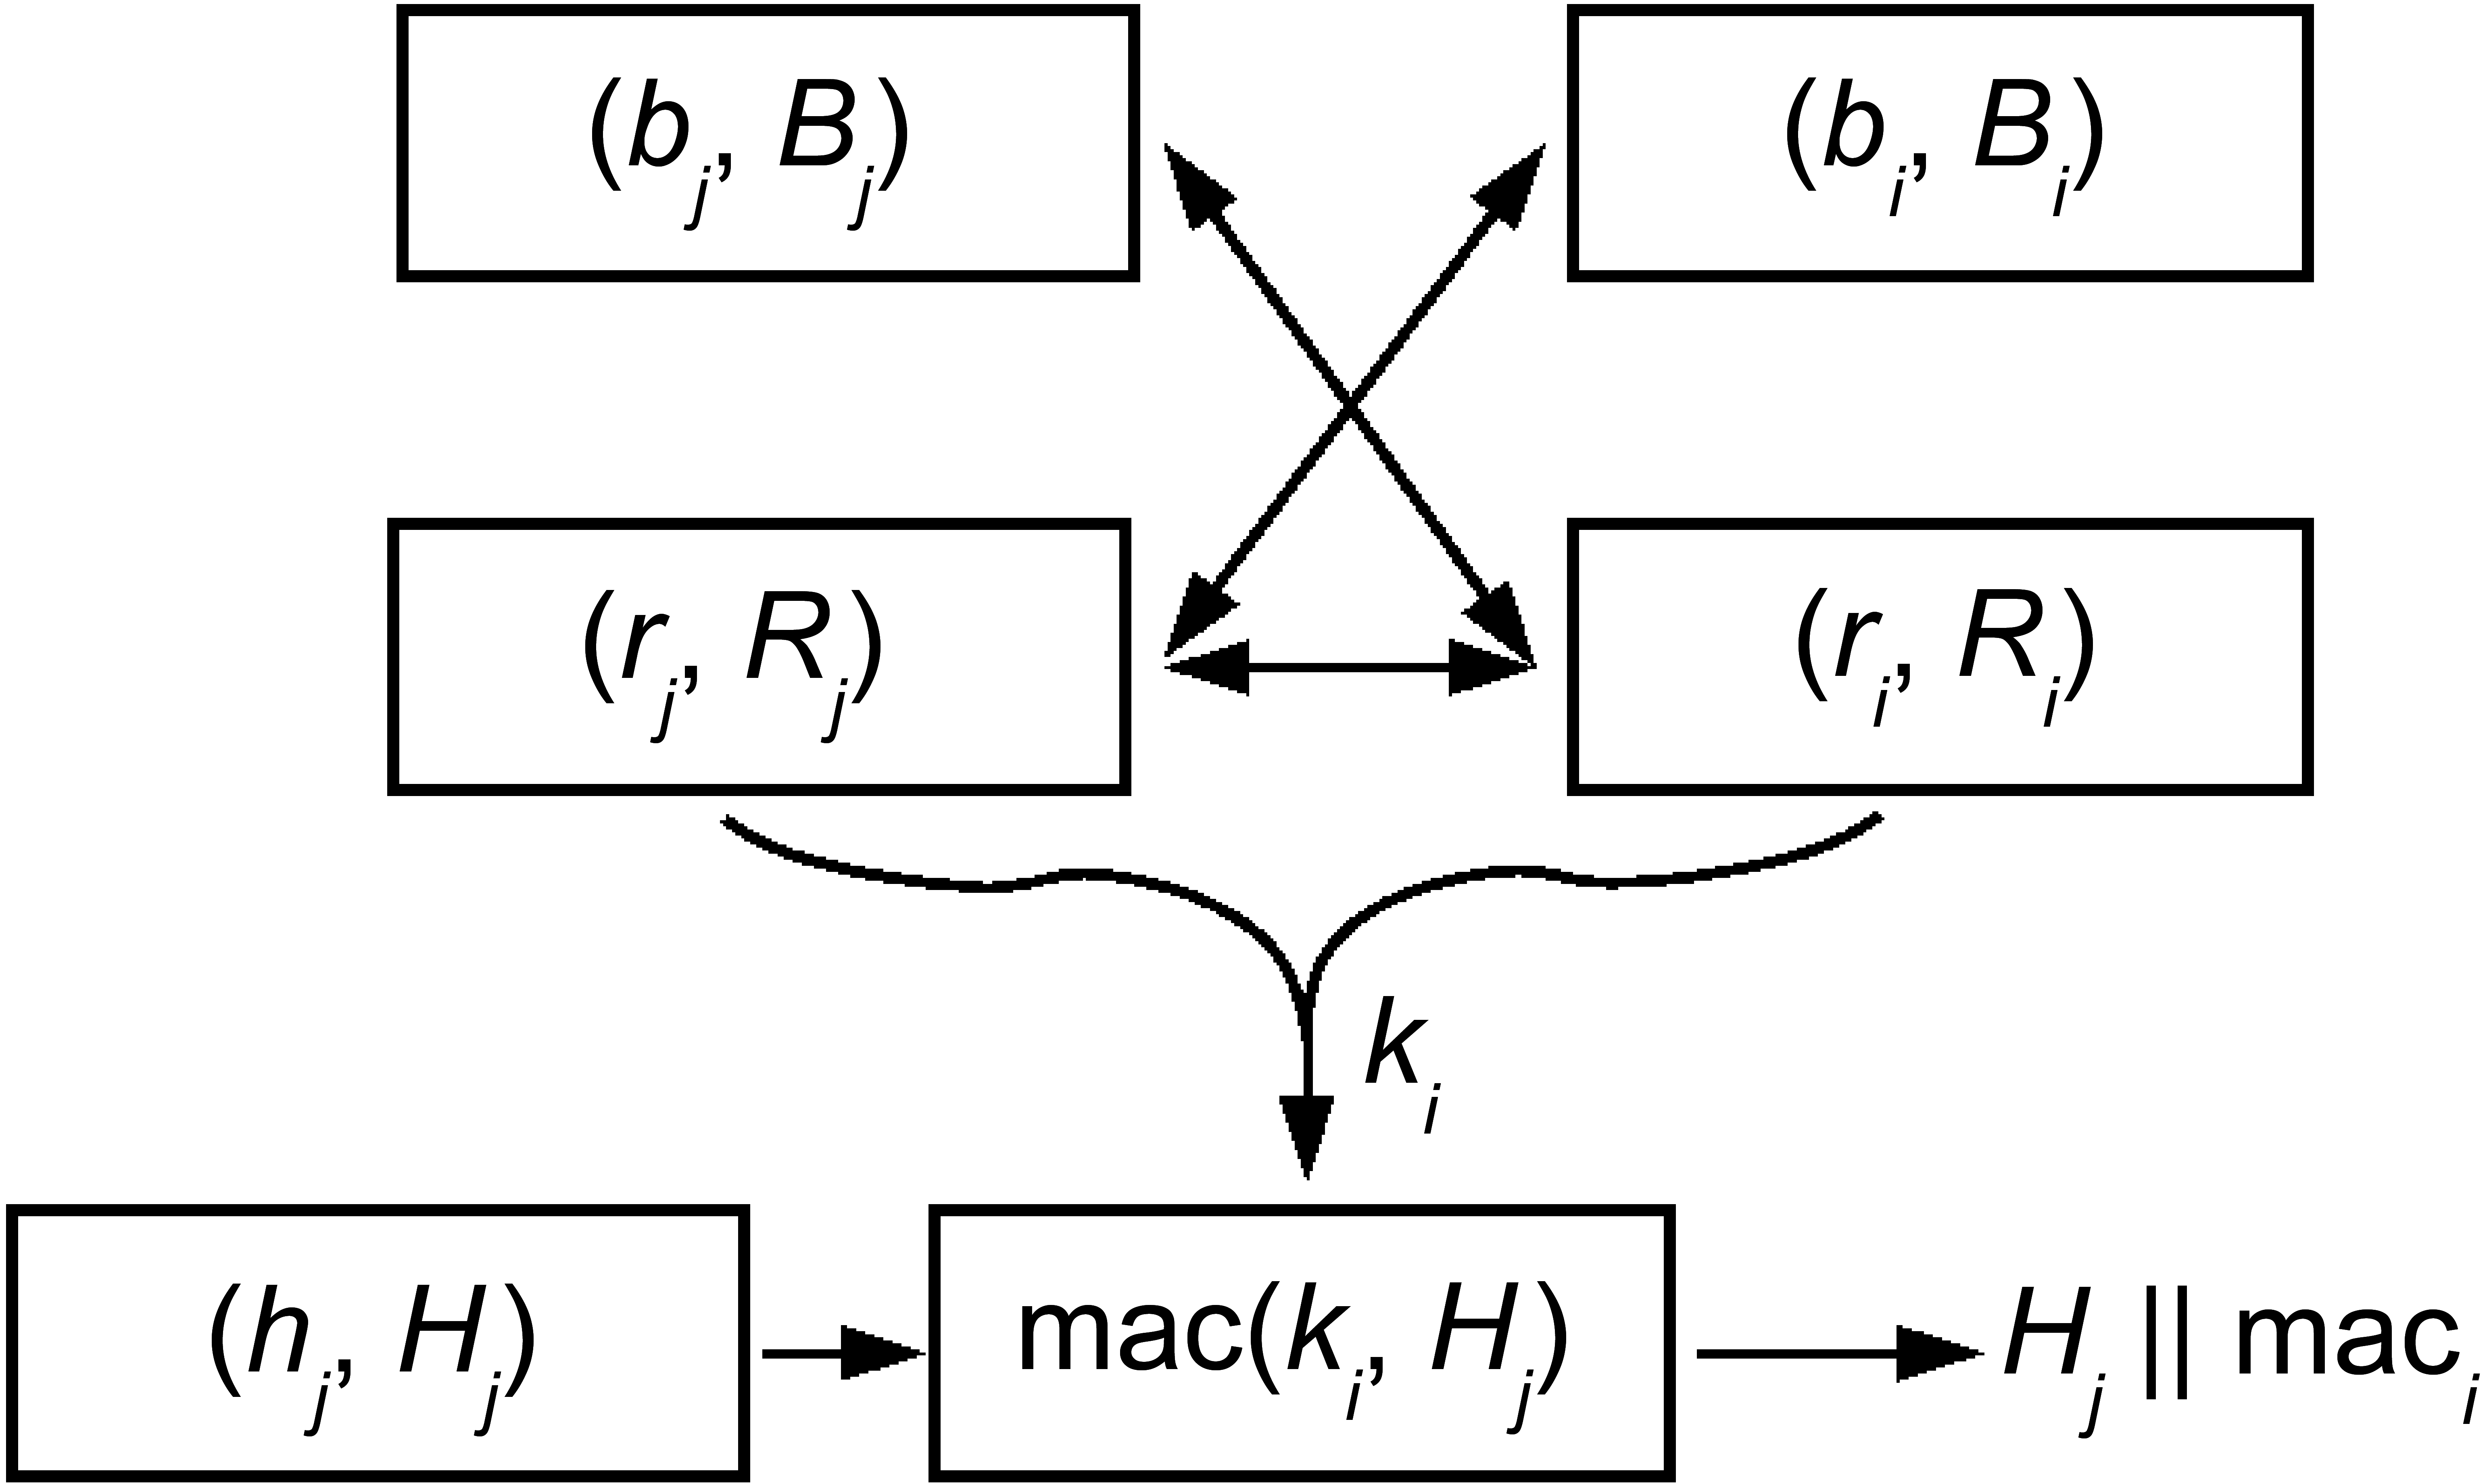
\includegraphics[width=6.5in]{key.eps}}
\caption{Triple Diffie-Hellman authenticated key exchange.}
\label{fig:exchange}
\end{figure}

\newpage
\begin{figure}[htb]
\centerline{\includegraphics[width=6.5in]{bd.eps}}
\caption{
Schematic illustration of the authenticated Burmester-Desmedt (BD) group key exchange
algorithm for a group of three participants, $A, B$, and $C$.
In the initial round, identity and ephemeral ratchet public keys are exchanged.
A triple DH key is then computed for each participant, and the BD handshake
public key mac is computed and attached to the BD handshake key, verifying its
authenticity.  The handshake public key, together with mac, is then exchanged in
a second round.
Using the public handshake keys, each participant computes his intermediate BD
key. This intermediate key is then exchanged in a third round, and the group
master key is computed by each user.}
\label{fig:bd}
\end{figure}

\end{document}
%
% ****** End of file apssamp.tex ******
